\section{Diseño y estructura del motor}

Antes de empezar a trabajar debemos conocer cómo vamos a comunicarnos con el motor gráfico y tener al menos una buena idea de la manera en que tratará la información que le proporcionemos.

\subsection{Ratio de fotogramas por segundo y bucle de ejecución}
\label{fps_bucle_ejecucion}
Aunque puede funcionar para la generación de imágenes estáticas, Manta es sobretodo un motor gráfico en tiempo real. Esto significa que su código se ejecuta múltiples veces para generar imágenes distintas y mostrarlas en pantalla, con lo cual se logra una ilusión de movimiento. De manera óptima suele considerarse como estándar los 60 fotogramas por segundo\cite{vsync_nvidia} (FPS o frames en adelante), aunque 24-30 FPS suele considerarse el mínimo aceptable. Debe tenerse en cuenta que aunque estos son los valores habituales, la tolerancia varía según el tipo de aplicación: en nuestro caso aunque buscamos una respuesta fluida, puede llegar a ser aceptable una bajada de los FPS sin afectar gravemente la experiencia de usuario.

Como implicación tenemos que para una buena experiencia en tiempo real todos los aspectos de la aplicación, incluyendo los cálculos de la propia aplicación como del propio motor y el renderizado a través de la GPU, deben calcularse como mínimo en unos $0.04$ segundos y óptimamente en $0.016$ segundos (los mencionados 24 y 60 FPS). En contraste, un render de alta calidad con ray tracing (una técnica que simula la física detrás de la interacción entre la luz y las superficies de un espacio) puede tardar varios minutos u horas\cite{nvidia_raytr}. Es de esperar por tanto que el motor sacrifique gran parte de ese realismo para reducir el tiempo de ejecución.

Para hacer esto de manera indefinida se encapsula todo el código del programa en un bucle de infinito que sólo puede detenerse manualmente y que contiene, en orden:

\begin{itemize}
    \item El cálculo del tiempo de ejecución del frame: las variaciones de FPS que puedan producirse a lo largo de la ejecución pueden provocar un efecto de aceleración y deceleración que empeora notablemente la experiencia. Además no se puede predecir cual será el ratio de FPS al que se ejecutará la aplicación cuando no conocemos en qué máquina se ejecutará y cual es su potencia. Para evitar este tipo de indeterminación calculamos el tiempo que transcurre entre un frame y el siguiente, el cual puede utilizarse en los cálculos a la hora de actualizar para compensar.
    \item La actualización de la aplicación: se llama una función desde la cual debemos actualizar la escena en función de los cálculos que realicemos. Cuando la aplicación alcance cierta complejidad, este puede llegar a ser el punto del bucle que absorba una mayor carga de trabajo, por lo que la eficiencia debe ser tenida en cuenta al actualizar para no ralentizar demasiado el programa.
    \item La actualización de la escena: Como se mencionará en el apartado \ref{scene_hierarchy}, el motor dispone de una colección de elementos que le hemos ordenado mostrar en pantalla. En este apartado se actualiza la escena para que refleje los cambios hechos en el proceso de actualización de la aplicación. Entre otras cosas, en este punto se calculan las transformaciones de las entidades (\ref{entity_component}) y se prepara toda la información que pueda necesitarse para renderizar.
    \item Renderizado: En este punto se envía toda la información necesaria a la GPU (incluyendo la cámara, las luces y los elementos de la escena) y se le ordena renderizar la escena. Aquí predomina el funcionamiento de la API gráfica, por lo que según la plataforma en que nos encontremos, este paso será realizado por una API diferente (véase el apartado \ref{APIS}).
\end{itemize}

Previamente al bucle se ejecutan las funciones de inicialización tanto del motor como de la aplicación, mientras que al detener la ejecución se libera la memoria reservada (normalmente durante esta primera inicialización).

\begin{figure}[H]
    \centering
    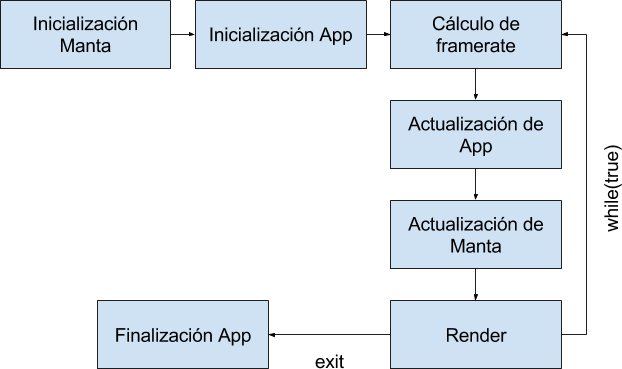
\includegraphics[scale=0.70]{Bucle}
    \caption{Esquema del bucle de ejecución.}
    \label{fig:bucle}
\end{figure}

\subsection{Patrón de entidad componente}
\label{entity_component}
En una aplicación 3D, podemos entender como entidad cualquier elemento que se encuentre en la escena. Por lo general todas tienen un elemento en común: tienen una transformación que indica su traslación, rotación y escalado. Sin embargo, cada entidad puede tener propósitos distintos: algunas son luces, otras cámaras, o objetos tridimensionales con malla y material, etc.

Dentro de cada categoría pueden haber varios tipos, o tal vez necesitamos que una entidad cumpla unas propiedades determinadas como emitir audio o verse afectada por un motor de físicas; y también podemos querer combinaciones de estas como que un elemento sea una luz y al mismo tiempo se balancee mediante un motor de físicas.

No queremos que nuestro código mezcle cosas tan dispares, tener las físicas y el audio en el mismo sitio resultaría en un código imposible de mantener a largo plazo; por lo que tenemos que buscar un modo de modularizar estas características. Para ello existe el patrón entidad-componente\cite{game_programming_patterns}, que nos permite crear componentes que aglomeran ciertas propiedades y comportamientos. Después podemos añadir cuantos componentes queramos a una entidad, permitiendo hacer que esta cumpla dichas propiedades sin aglomerar todo el código de estas.

Para implementar este patrón tenemos dos clases principales "Entity" y "Component", las cuales podremos extender como deseemos para crear distintos tipos de cada una. Una entidad por defecto contiene una lista de componentes, que en el fondo son instancias de los diferentes tipos de componentes que creemos. Component es una clase abstracta y sus clases derivadas deben implementar uno o varios métodos que puedan ser llamados desde la entidad.

De este modo, cada vez que la entidad necesite delegar una funcionalidad a sus componentes, iterará sobre ellos y llamará dichos métodos, que tendrán un comportamiento distinto según se requiera. En nuestro caso, los métodos que implementa Component son los siguientes:

\begin{itemize}
    \item AddedToEntity: Llamado en el momento en que se incorpora el componente a la entidad.
    \item RemovedFromEntity: Llamado en el momento en que este se borra de la entidad (lo cual normalmente significa que estamos eliminando la entidad, pero no necesariamente).
    \item AddedComponent: Se llama a todos los componentes que tenga la entidad cada vez que se añade uno nuevo, e incluye una referencia por parámetro del componente añadido.
    \item RemovedComponent: Al igual que la anterior, cuando se elimina un componente también se hace saber al resto de componentes aún existentes.
\end{itemize}

Aunque no lo hemos utilizado, es bastante típico en el patrón Component tener un método "update" que se llama en cada actualización de la aplicación (\ref{fps_bucle_ejecucion}) y hace que las propias entidades se encarguen de su propio comportamiento en tiempo real, a través de los componentes. Nosotros no hemos implementado esta capacidad porque hemos decidido que sean funciones externas quienes controlen dicho comportamiento, y no las propias entidades.

Para acceder externamente a los compoentes, en la clase Entity hacemos uso de "templates" de C++, sobre los cuales no vamos a profundizar. Los templates permiten implementar un método independientemente del tipo de las variables con las que trabaja, de modo que este tipo se especifica en el momento de llamar al método. Para pedirle a una entidad que nos dé acceso a un componente específico, le podemos especificar el tipo del componente que queremos y desde el método buscar qué componentes son de dicho tipo.

\subsection{Escena, jerarquía y pasos previos al renderizado}
\label{scene_hierarchy}
Como se ha mencionado en el apartado \ref{entity_component}, disponemos de una serie de entidades distribuidas por el espacio con una traslación, rotación y escalado. Este espacio se conoce como la escena.

Al crear una entidad, esta automáticamente se registra a sí misma en la jerarquía de la escena. La jerarquía contiene por tanto un listado con punteros a cada una de las entidades que le permite acceder a sus componentes. El motor trabaja directamente con este listado de objetos y hará directamente todo lo que se requiera con ellos dependiendo de sus componentes. Por lo tanto, el usuario no debe pedir en ningún momento que se rendericen los objetos: basta con crear una entidad que tenga un componente de malla (véase el apartado \ref{mesh_light_cam}) para que el motor entienda que deberá renderizarlo.

Las entidades están organizadas en la jerarquía de tal modo que una entidad puede ser padre de otras entidades, formando una estructura de árbol. Las transformaciones de las entidades se acumulan desde la raíz de la jerarquía hacia abajo, es decir: si una entidad está desplazada o rotada, sus entidades "hijas" tendrán una traslación y rotación respecto a la primera. Esto permite crear diferentes estructuras dentro de la escena y trabajar con estas sin tener que controlar la posición de todos los elementos que la componen. Por ejemplo: si tenemos una entidad "coche" y otra entidad "asientos" asignar el primero como padre de los segundos hará que se mantengan en su sitio, pegados a la estructura del coche, dado que su transformación es relativa a este.

Una consecuencia de este sistema es que las transformaciones que tenemos en cada entidad no son realmente la transformación respecto al centro de la escena, que es la que necesitamos en el momento de renderizar. Por lo tanto debemos realizar un cálculo previo al renderizado que consiste en multiplicar las transformaciones en cada una de las ramas de la escena y asignarlas a cada uno de los elementos.

\subsection{Mallas, luces y cámara}
\label{mesh_light_cam}
Se trata de los ejemplos más importantes de componentes (véase el apartado \ref{entity_component}) que se utilizan en el motor.

\subsubsection{Mallas}
Entendemos por malla (o mesh) un listado de vértices conectados por otro listado de índices. Los vértices contienen información de la posición, normal, tangente, bitangente y coordenadas UV (véase \ref{materials}) mientras que los índices simplemente ordenan los vértices de 3 en 3 creando triángulos. Los componentes "MeshComponent" y "MeshDynamicComponent" recogen esta información para que el motor renderice el resultado posteriormente. Estos componentes también incluyen los materiales de las mallas.

La diferencia principal entre ellos es que "MeshComponent" lee los datos de un fichero al crearse y es inmutable, mientras que "MeshDynamicComponent" se crea asignando una cantidad máxima de vértices e índices y estos se asignan programáticamente, pudiendo modificarse en cualquier momento (será muy importante para la generación dinámica de paredes y ventanas en la sección \ref{walls_holes}). Otra diferencia importante es que "MeshComponent" puede contener diversas sub-mallas que comparten transformación pero pueden tener distintos materiales, mientras que "MeshDynamicComponent" solo puede contener una.

\subsubsection{Luces}
Las luces son el elemento más complejo de un motor gráfico. La calidad de la luz es el elemento que más influye en el realismo de la imagen generada, y es uno de los puntos que más coste computacional requiere. En las técnicas de renderizado de alta calidad, se trata de simular la física de la luz para conseguir un gran realismo, pero esto es impracticable en un motor en tiempo real como se ha dicho en el apartado \ref{fps_bucle_ejecucion}.

En el momento de renderizar se utilizan luces para saber con qué intensidad debe renderizarse cada elemento de la escena, o los diferentes puntos de su superficie. Conociendo en qué dirección incide la luz y la normal de la superficie en el punto que queremos pintar, mediante el producto escalar de estos vectores podemos saber si la luz incide sobre este punto y con qué intensidad. Además las luces pueden tener color (normalmente será luz blanca pero no tiene por qué ser así) que se refleja mezclando el color de la luz con el de la superficie.

En la realidad las luces pueden tener formas muy variadas, pero en el motor se reducen a: puntos de luz, luces direccionales, focos, luces de área, luces esféricas y luces cilíndricas. El tipo de luz hará variar el modo en que incide sobre la escena. Las propiedades de esta se asignan en el momento de crear el componente y pueden cambiarse en cualquier momento.

\subsubsection{Cámara}
La cámara indica el punto de vista desde el que se realizará el renderizado de la escena. Existen dos tipos (fig. \ref{fig:camera}):

\begin{itemize}
    \item Cámara ortogonal: se caracteriza por mostrar todos los elementos con la misma escala, sin importar la distancia en que estén. Es especialmente útil para comparar tamaños de distintos elementos, y la utilizaremos para vistas superior y frontales de la habitación, pensados como modos de edición de esta. Sus propiedades son el tamaño, en alto y ancho, de su campo de visión.
    \item Cámara en perspectiva: imita el modo en que vemos los objetos en la realidad, teniendo en cuenta la distancia en que se encuentran. Da resultados mucho más satisfactorios para visualizar la habitación, y transmite más información espacial. Sus propiedades son el ángulo de su campo de visión, más conocido como FOV (field of view), y los planos cercano y lejano de este, comúnmente conocidos como near plane y far plane.
\end{itemize}

\begin{figure}[H]
    \centering
    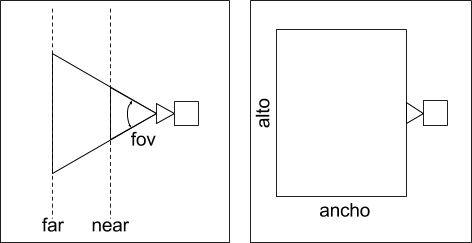
\includegraphics[scale=0.75]{camera}
    \caption{Diferencias entre una cámara en perspectiva y ortogonal, respectivamente.}
    \label{fig:camera}
\end{figure}

\subsection{Materiales}
\label{materials}
El material de un objeto 3D describe el aspecto que ha de tener la superficie de este en el momento de renderizarlo. Para conseguirlo se asocian una serie de texturas del mismo tamaño y se asocia cada uno de los vértices con coordenadas de dos componentes dentro de estas texturas (conocidas como UV, véase \ref{mesh_light_cam}). Como se explica en el apartado \ref{shaders}, el shader interpola los datos entre dos vértices a cada uno de los píxeles intermedio. De este modo sabiendo la UV que corresponde a cada uno de los vértices podemos saber la que corresponde a cada píxel del objeto 3D.

Las texturas que forman el material pueden ser un color único (que equivale a aplicar una textura de ese color o una imagen importada desde un fichero. El material está formado por los siguientes tipos de texturas o mapas:

\begin{itemize}
    \item Albedo: En el terreno de la física, el albedo es la cantidad de luz que rebota sobre una superficie tras incidir sobre esta\cite{def_albedo}. En nuestro caso podemos entenderlo como la textura que expresa el color que ha de tener la superficie en cada punto.
    \begin{figure}[H]
        \centering
        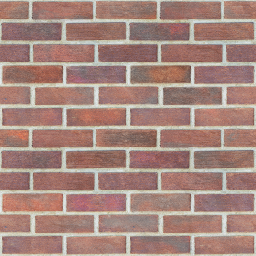
\includegraphics[width=0.4\linewidth]{material_example/albedo_example}
        \caption{Ejemplo de Albedo\cite{free_pbr}.}
        \label{fig:albedo_ex}
    \end{figure}
    \item Mapa de normales: Habitualmente, la normal de la superficie se expresa a partir de la propia geometría de esta, pero a veces queremos ciertos detalles que requerirían aumentar mucho la resolución de la malla, aumentando con ello también el peso del modelo 3D y el coste computacional de procesar y renderizar dicha información. Para evitar esto podemos utilizar una textura de normales: en cada píxel, a la normal de la superficie que hemos interpolado a partir de los vértices próximos, le sumamos la normal correspondiente extraída del mapa de normales. Esto permite crear un efecto de profundidad o rugosidad sin modificar la geometría del objeto.
    \begin{figure}[H]
        \centering
        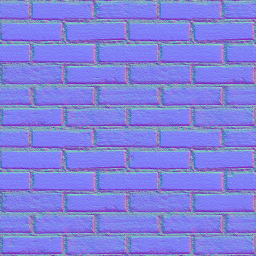
\includegraphics[width=0.4\linewidth]{material_example/normal_map_example}
        \caption{Ejemplo de Mapa de Normales\cite{free_pbr}.}
        \label{fig:normal_map_ex}
    \end{figure}
    \item Aspereza (roughness): Se produce cuando la superficie tiene micro-imperfecciones que afectan a los reflejos, haciendo que se difuminen. Cuanto mayor sea la aspereza, más se dispersará la luz al rebotar contra la superficie, y más se difuminará el reflejo; mientras que en una superficie sin imperfecciones la luz se reflejará uniformemente.
    \begin{figure}[H]
        \centering
        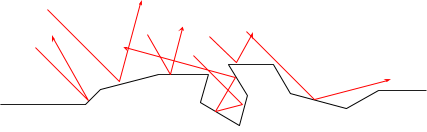
\includegraphics[width=0.6\linewidth]{material_example/roughness_example}
        \caption{El roughness simula las micro-imperfecciones de la superficie.}
        \label{fig:roughness_ex}
    \end{figure}
    \item Fresnel\cite{marmoset_basicpbr}: El reflejo Fresnel (nombre que hace referencia a su descubridor, Augustin-Jean Fresnel) es la propiedad según la cual los materiales reflejan más cuanto más grande es el ángulo entre la normal de la superfície y la dirección de la luz.
    %\item Reflejo Anisotrópico\cite{anisotropic_ref}: Se produce cuando la superfície tiene imperfecciones organizadas en un patrón, de manera que el ángulo desde el que observamos hace variar el reflejo resultante. Se hace especialmente evidente en metales pulidos, ciertos tejidos, pelo o grandes superficies de agua.
    \item Metalizado\cite{marmoset_basicpbr}: Los metales tienden a reflejar la luz, razón por la que se define un valor de metalizado para especificar la cantidad de luz que refleja una superficie. Con el metalizado también se puede definir un tinte para la luz reflejada (por ejemplo, reflejos amarillentos en la superficie del oro).
    \item Oclusión ambiental\cite{ambient_occlusion}: Se trata de un efecto del que a menudo se abusa, dado que no existe en la realidad. El mapa de oclusión permite oscurecer ciertas zonas de la geometría, normalmente los puntos que forman ángulos más cerrados. Resulta efectivo para imitar ciertas sombras que se producen en estos puntos, pero en exceso puede resultar artificial.
    \begin{figure}[H]
        \centering
        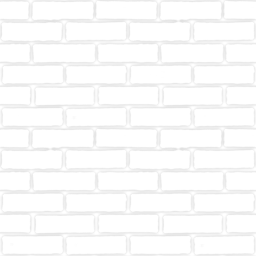
\includegraphics[width=0.4\linewidth]{material_example/ambient_occlussion_example}
        \caption{Ejemplo de mapa de oclusión ambiental.}
        \label{fig:occlusion_ex}
    \end{figure}
\end{itemize}

\subsection{Gestión de memoria}
Una de las operaciones que más tiempo demandan en C++ es solicitar nueva memoria al sistema operativo. Debido a eso, abusar de las asignaciones de memoria, por ejemplo haciéndolas dentro de bucles (como el bucle de Manta), puede hacer que el programa se ralentice considerablemente.

Para minimizar la cantidad de asignaciones que realizamos, manta tiene un único "bloque de memoria" (más conocido como memory pool). El memory pool asigna una gran cantidad de memoria al inicializar el programa y nos da acceso a esta cada vez que lo necesitemos. En caso de no necesitar más dicha memoria, podemos solicitar al memory pool que la libere, dejándola disponible en adelante. Hacer esto es computacionalmente gratuito, de modo que no necesitamos preocuparnos de las asignaciones que necesitemos hacer.

Sin embargo, existen dos desventajas importantes:

Por un lado necesitamos saber desde el principio cuánta memoria podemos llegar a necesitar dado que esta solo se va a asignar una vez; en caso de superar ese límite de memoria tendremos un error de segmentación que detendrá el programa.

Por otro lado, también necesitamos tener mucho más cuidado con la memoria que solicitemos al memory pool: si nos equivocamos al manejar la memoria asignada, C++ suele responder con un error de segmentación; pero si hacemos lo mismo con la memoria del memory pool, ese error no se producirá y estaremos modificando datos que corresponden a otras variables. Al fin y al cabo, el puntero que recibimos a punta a una posición desconocida del memory pool, y nada nos impide desplazarnos por este sin tener en cuenta el tamaño de la memoria que nos ha asignado.
